\documentclass[11pt, oneside]{article}   	% use "amsart" instead of "article" for AMSLaTeX format
\usepackage{geometry}                		% See geometry.pdf to learn the layout options. There are lots.
\geometry{letterpaper}                   		% ... or a4paper or a5paper or ... 
%\geometry{landscape}                		% Activate for for rotated page geometry
%\usepackage[parfill]{parskip}    		% Activate to begin paragraphs with an empty line rather than an indent
\usepackage{graphicx}				% Use pdf, png, jpg, or eps§ with pdflatex; use eps in DVI mode
								% TeX will automatically convert eps --> pdf in pdflatex		
\usepackage{amssymb}
\usepackage{amsmath}
\usepackage{parskip}
\usepackage{hyperref}

\title{Improper integrals}
%\author{The Author}
%\section{}
% \subsection*{R code}
\date{}							% Activate to display a given date or no date

\graphicspath{{/Users/telliott_admin/Dropbox/Tex/png/}}

\begin{document}
\maketitle
\Large
\noindent
Strang:
An "improper" integral is one in which some part of $\int_a^b y(x) \ dx$ becomes \emph{infinite}.  It might be $b$ or $a$ or the function $y$.  The region under the graph reaches infinitely far---to the right or left or up or down.  (Those come from $b = \infty$ and $a = -\infty$ and $y \Rightarrow \infty$ and $y \Rightarrow -\infty$).  Nevertheless the integral may "converge".  Just because the region is infinite, it is not automatic that the area is infinite.

Here are three examples:
\[ \int_1^\infty \frac{1}{x^2} \ dx = - \frac{1}{x} \ \bigg |_1^\infty = 1 \]
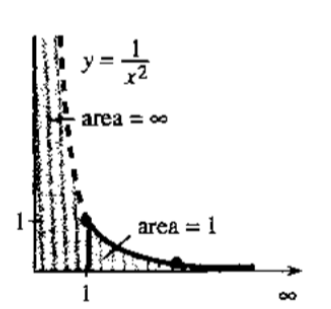
\includegraphics [scale=0.5] {improper2.png}
\[ \int_{-\infty}^0 e^x \ dx = e^x \ \bigg |_{-\infty}^0 = 1 \]
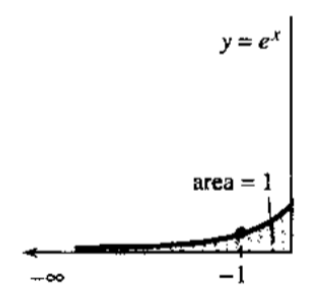
\includegraphics [scale=0.5] {improper3.png}
\[ \int_0^1 \frac{1}{\sqrt{x}} \ dx = 2 \sqrt{x} \ \bigg |_0^1 = 2 \]
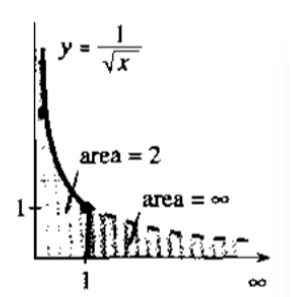
\includegraphics [scale=0.5] {improper4.png}

Two more:
\[ \int_1^\infty \frac{1}{x} \ dx = \ln{x} \ \bigg |_1^\infty = \infty \]
\[ \int_1^\infty \frac{1}{x^p} \ dx = \frac{x^{1-p}}{1-p} \ \bigg |_1^\infty = \frac{1}{p-1} \]

The last one is finite \emph{if} $p > 1$.

\end{document}  